\documentclass[11pt]{article}
\usepackage[margin=1in]{geometry}
\usepackage{amsmath,amssymb,amsthm,mathtools}
\usepackage{booktabs,tabularx,array}
\usepackage{float}
\usepackage{graphicx}
\usepackage{xcolor}
\usepackage{microtype}
\usepackage[hidelinks]{hyperref}
\allowdisplaybreaks[2]

\newtheorem{theorem}{Theorem}
\newtheorem{proposition}[theorem]{Proposition}
\newtheorem{lemma}[theorem]{Lemma}
\newtheorem{corollary}[theorem]{Corollary}
\theoremstyle{definition}
\newtheorem{definition}[theorem]{Definition}
\theoremstyle{remark}
\newtheorem{remark}[theorem]{Remark}

\newcommand{\Bd}{\mathrm{Bd}}
\newcommand{\dB}{\mathrm{dB}}
\newcommand{\rhoU}[3]{\rho_{#1}(#2,#3)}
\newcommand{\Rsim}{R_{\mathrm{sim}}}
\newcommand{\eps}{\varepsilon}
\newcommand{\one}{\mathbf{1}}
\newcommand{\openstatus}{%
  \begin{center}
  \fbox{\parbox{0.91\textwidth}{\centering
  \textbf{Scope.}  This paper proves the lower bound
  $\Rsim\geq 3/2$ and the exact interval of one explicit family.
  A universal upper bound and the exact value of $\Rsim$ remain \textbf{open}.}}
  \end{center}}

\title{A fitness-independent family of simultaneous amplifiers\\
below fitness three halves}
\author{Alec Kriebel\\Independent Researcher}
\date{August 8, 2026}

\begin{document}
\maketitle

\begin{abstract}
We study fixation from a uniformly random single mutant on finite connected
loopless undirected weighted graphs under both Birth--death (Bd) and
death--Birth (dB) Moran updating.  We construct one explicit family, with
positive rational weights independent of mutant fitness, whose fixation
probability converges to $1/3$ under both rules for every fixed fitness
$r>1$.  Since the corresponding complete-graph probabilities converge to
$1-1/r$, the family strictly amplifies both rules for every fixed
$1<r<3/2$ once the population is sufficiently large.  Thus the asymptotic
simultaneous-amplification threshold satisfies $R_{\mathrm{sim}}\geq3/2$.
The proof solves the singular three-vertex module exactly, derives a marked
rare-edge trace with explicit coupling error, and controls both the initial
module-to-center transition and the subsequent center sweep.  At $r=3/2$
we retain the order-$N^{-2}$ terms and prove that this same family suppresses
both rules.  Hence $(1,3/2)$ is the exact amplification interval of the
constructed family.  We also give an exact unweighted graph on 36 vertices
which refutes two stronger candidate endpoint separators: both the normalized
fixation product and the balanced normalized arithmetic mean exceed one.  A
growing clique--pendant family strengthens this to a nonvanishing product
violation, with normalized limits $32/27$ and $8/9$.  Varying its leaf
proportion proves that every universal convex affine separator must give Bd
coefficient at most $1/3$; this upper bound is sharp among all such
separators.  The sharp one-third inequality itself remains open.  All
counterexamples here suppress dB, so no universal upper bound, and therefore
no exact value of $R_{\mathrm{sim}}$, is claimed.
\end{abstract}

\openstatus

\section*{Author summary}

An amplifier is a population structure on which a beneficial mutation is
more likely to take over than in a well-mixed population of the same size.
The two standard update orders---choosing birth first or death first---often
favor different structures.  We give one sequence of weighted graphs that
works for both update orders throughout the entire fixed-fitness interval
$1<r<3/2$.  Each graph has a small central clique and many almost isolated
three-vertex modules.  A mutation usually starts in a module, where it has
asymptotic chance $1/3$ to occupy the module.  A carefully separated set of
edge scales then makes an occupied module seed the center and makes an
occupied center sweep the remaining modules, both with probability tending
to one.  Exact formulas and explicit error estimates turn this timescale
picture into a proof.  The construction fails at the endpoint $r=3/2$ by a
computed order-$N^{-2}$ deficit.  Whether some different family reaches or
passes that endpoint remains open.  An exact 36-vertex calculation included
below shows, however, that neither the normalized product nor the balanced
arithmetic mean can serve as the universal endpoint separator.  A growing
version explains the sharp remaining affine weights: Bd can gain
asymptotically two units for each unit lost by dB, making $1:2$ the maximal
possible Bd:dB weight ratio.

\section{Introduction}

For a fixed population size, a graph is a simultaneous amplifier at fitness
$r$ if it increases uniformly initialized fixation probability, relative to
the complete graph, under both Bd and dB updating.  The large-population
question has a delicate order of quantifiers: one graph family must be
chosen independently of $r$, but the population size from which amplification
holds may depend on $r$.  A previous weighted modular construction established
simultaneous amplification on the interval $(1,1.2)$
\cite{Svoboda2024}.  The present construction extends the rigorous lower
endpoint benchmark to $3/2$.

The mechanism is a singular three-scale hierarchy.  A module is a weighted
triangle with one edge of weight one and two edges of weight
$\delta_N=N^{-4}$.  There are $N^2$ modules.  The center is a clique of $N$
vertices with edge weight $z_N=N^{-3}$, and every center--module edge has the
much smaller rational weight $\eps_N=N^{-N^3}$.  The very small final scale
does not itself create the bias.  Rather, it separates internal absorption
from intercomponent motion sufficiently strongly that an exact marked trace
approximates the original chain through all polynomially many excursions.

Two comparisons drive the trace.  Starting from a mutant module, the odds of
fixing a mutant in the center before erasing the module grow as a positive
constant times $N^2$ for each rule.  Once the center is mutant, the chance of
a resident module reversing it is exponentially small, while all $N^2$
modules are converted in only polynomially many trace excursions.  The
isolated triangle therefore determines the limiting fixation probability,
and its uniformly averaged value tends to $1/3$ under both rules.

The proof also explains why the endpoint requires a separate calculation.
For $r<3/2$, a positive constant gap separates $1/3$ from the complete-graph
limit.  At $r=3/2$ that gap vanishes, so we compute the first-stage failure
probability, the center-start contribution, and the finite complete-graph
correction through order $N^{-2}$.  Both comparisons are then strictly
negative.  This establishes the exact interval for this family only.

\section{Model, baselines, and the asymptotic threshold}

Let $G=(V,w)$ be a finite connected loopless undirected weighted graph,
$|V|=n$, with
\[
 w_{uv}=w_{vu}\geq0,\qquad w_{uu}=0,
 \qquad d_u:=\sum_v w_{uv}>0.
\]
A state is the mutant set $S\subseteq V$.  Mutants have fitness $r>1$ and
residents have fitness one.  Put $F(S)=r|S|+n-|S|$.

Under Bd updating, first a parent is chosen proportional to fitness and then
one of its replacement targets is chosen proportional to the incident edge
weight.  Thus, for $v\notin S$ and $v\in S$, respectively,
\begin{align}
 P_{\Bd}(S,S\cup\{v\})
 &=\frac{r}{F(S)}\sum_{u\in S}\frac{w_{uv}}{d_u},
 \label{eq:Bd-up}\\
 P_{\Bd}(S,S\setminus\{v\})
 &=\frac{1}{F(S)}\sum_{u\notin S}\frac{w_{uv}}{d_u}.
 \label{eq:Bd-down}
\end{align}
Under dB updating, first a uniformly chosen vertex dies and then a neighbor
is chosen proportional to fitness times edge weight.  Hence
\begin{align}
 P_{\dB}(S,S\cup\{v\})
 &=\frac1n\frac{r\sum_{u\in S}w_{uv}}
 {r\sum_{u\in S}w_{uv}+\sum_{u\notin S}w_{uv}},
 &&v\notin S,\label{eq:dB-up}\\
 P_{\dB}(S,S\setminus\{v\})
 &=\frac1n\frac{\sum_{u\notin S}w_{uv}}
 {r\sum_{u\in S}w_{uv}+\sum_{u\notin S}w_{uv}},
 &&v\in S.\label{eq:dB-down}
\end{align}
The remaining probability is a self-loop.  With $h_U(S)$ denoting fixation
probability from $S$, these transition probabilities determine the unique
solution of
\[
 h_U(S)=\sum_TP_U(S,T)h_U(T),\qquad
 h_U(\varnothing)=0,\qquad h_U(V)=1.
\]
We use uniform singleton initialization:
\[
 \rho_U(G,r):=\frac1n\sum_{v\in V}h_U(\{v\}),
 \qquad U\in\{\Bd,\dB\}.
\]

\subsection{Complete-graph baselines}

On the unit-weight complete graph $K_n$, the mutant count is a birth--death
chain.  For Bd the adjacent down/up ratio is $1/r$, and the standard
one-dimensional harmonic recurrence gives
\begin{equation}
 \rho_{\Bd}(K_n,r)=\frac{1-r^{-1}}{1-r^{-n}}.
 \label{eq:complete-Bd}
\end{equation}
For dB, let $T_i^+$ and $T_i^-$ be the probabilities that the mutant count
moves from $i$ to $i+1$ and $i-1$.  Direct substitution in
\eqref{eq:dB-up}--\eqref{eq:dB-down} gives the telescoping product
\[
 \prod_{j=1}^{i}\frac{T_j^-}{T_j^+}
 =\frac{n-1+(r-1)i}{(n-1)r^i}.
\]
Substitution into the birth--death-chain fixation formula yields
\begin{equation}
 \rho_{\dB}(K_n,r)
 =\frac{n-1}{n}\frac{1-r^{-1}}{1-r^{-(n-1)}}.
 \label{eq:complete-dB}
\end{equation}
For each fixed $r>1$, both expressions converge to
\begin{equation}
 q(r):=1-\frac1r.
 \label{eq:q}
\end{equation}

\subsection{The order of quantifiers}

\begin{definition}
Let $R_{\mathrm{sim}}$ be the supremum of all $R>1$ for which there exists a
single family $\{G_m\}$, with $|V(G_m)|\to\infty$ and weights independent of
fitness, such that
\[
 \forall r\in(1,R)\ \exists m_0(r)\ \forall m\geq m_0(r):
 \quad
 \rho_{\Bd}(G_m,r)>\rho_{\Bd}(K_{|V(G_m)|},r)
\]
and simultaneously
\[
 \rho_{\dB}(G_m,r)>\rho_{\dB}(K_{|V(G_m)|},r).
\]
\end{definition}

The threshold $m_0(r)$ need not be uniform as $r\downarrow1$ or as $r$
approaches the upper endpoint.  None of the limits below interchanges those
quantifiers.

\section{The center--triangle family and main theorem}

For each integer $N\geq3$, put
\begin{equation}
 c_N=N,\qquad M_N=N^2,\qquad
 \delta_N=N^{-4},\qquad z_N=N^{-3},\qquad
 \eps_N=N^{-N^3}.
 \label{eq:scales}
\end{equation}
The graph $G_N$ has a center set $C_N$ of $c_N$ vertices and $M_N$ disjoint
three-vertex modules.  In module $j$, with vertices $A_j,B_j,D_j$, set
\begin{equation}
 w(A_j,D_j)=1,\qquad
 w(A_j,B_j)=w(B_j,D_j)=\delta_N.
 \label{eq:module-weights}
\end{equation}
Every pair of distinct center vertices has weight $z_N$.  Every center vertex
is joined to every module vertex by an edge of weight $\eps_N$.  There are no
edges between distinct modules.  Therefore
\begin{equation}
 n_N:=|V(G_N)|=N+3N^2.
 \label{eq:order}
\end{equation}
All displayed weights are positive rational numbers, $G_N$ is connected,
and the construction is independent of $r$.

\begin{figure}[t]
 \centering
 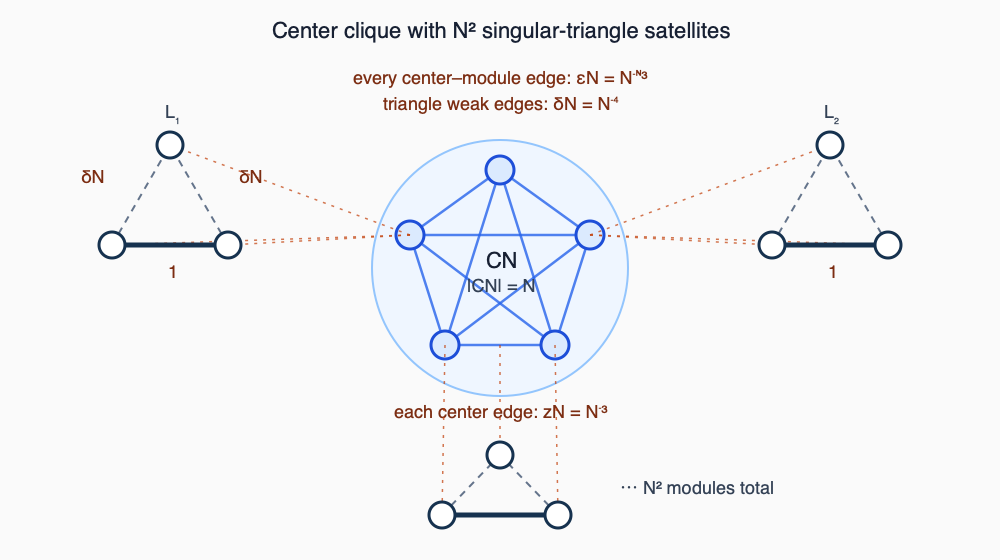
\includegraphics[width=0.97\textwidth]{assets/center_triangle_diagram.png}
 \caption{The center clique and three representative singular-triangle
 modules.  Every center is joined to every module vertex by an
 $\eps_N$-edge; only representative outer edges are drawn.}
 \label{fig:construction}
\end{figure}

\begin{theorem}[Simultaneous amplification below three halves]
\label{thm:main}
For each fixed $r>1$,
\begin{equation}
 \lim_{N\to\infty}\rho_{\Bd}(G_N,r)
 =\lim_{N\to\infty}\rho_{\dB}(G_N,r)=\frac13.
 \label{eq:main-limit}
\end{equation}
Consequently, for every fixed $1<r<3/2$, both strict complete-graph
comparisons hold for all sufficiently large $N$.  In particular,
\[
 R_{\mathrm{sim}}\geq\frac32.
\]
For this particular family, $(1,3/2)$ is the exact asymptotic fixed-fitness
amplification interval.  At the endpoint,
\begin{align}
 \rho_{\Bd}(G_N,3/2)-\rho_{\Bd}(K_{n_N},3/2)
 &=-\frac{4}{3N^2}+o(N^{-2}),\label{eq:end-Bd}\\
 \rho_{\dB}(G_N,3/2)-\rho_{\dB}(K_{n_N},3/2)
 &=-\frac{16}{81N^2}+o(N^{-2}).\label{eq:end-dB}
\end{align}
For every fixed $r>3/2$, the family eventually suppresses both rules.
\end{theorem}

The rest of the paper proves the theorem.  Equations
\eqref{eq:end-Bd}--\eqref{eq:end-dB} do not imply a universal obstruction at
$r=3/2$.

\section{Exact calculation on one singular triangle}

Write $H_\delta$ for one module with $\delta>0$, and label the middle vertex
of the two weak edges by $B$.  Its weighted degrees are
\begin{equation}
 d_A=d_D=1+\delta,\qquad d_B=2\delta.
 \label{eq:triangle-degrees}
\end{equation}
For $U\in\{\Bd,\dB\}$, let $f_v^U(\delta,r)$ be fixation in $H_\delta$
from a mutant at $v$, and define
\[
 \alpha_U(\delta,r)=\frac13\sum_{v\in\{A,B,D\}}f_v^U(\delta,r).
\]
Let $\beta_v^U(\delta,r)$ be fixation of a single resident at $v$ in an
otherwise mutant module.  After multiplying all fitnesses by $1/r$, this is
$f_v^U(\delta,1/r)$.

For completeness, the exact calculation uses all six nonabsorbing subsets
$S\subset\{A,B,D\}$.  In each such state one inserts the three edge weights
in \eqref{eq:Bd-up}--\eqref{eq:dB-down}, removes the self-loop, and solves
\begin{equation}
 \left(\sum_{T\ne S}P_U(S,T)\right)h_U(S)
 -\sum_{\varnothing\ne T\ne S,\,T\ne V}P_U(S,T)h_U(T)
 =P_U(S,V).
 \label{eq:six-state-system}
\end{equation}
Reflection $A\leftrightarrow D$ reduces the six unknowns to four, although
the independent verifier retains all six.  Direct elimination gives the
following rational expressions.

Set
\begin{align*}
D_B={}&9r^2
+\delta(12r^4+24r^3+15r^2+24r+12)\\
&+\delta^2(16r^4+52r^3+83r^2+52r+16)\\
&+\delta^3(4r^4+12r^3+13r^2+12r+4).
\end{align*}
Then
\begin{equation}
 \alpha_{\Bd}
 =\frac{r^2\{3+\delta(12r^2+12r+5)
 +\delta^2(16r^2+36r+21)
 +\delta^3(4r^2+8r+3)\}}{D_B},
 \label{eq:alpha-Bd}
\end{equation}
and
\begin{equation}
 \alpha_{\dB}
 =\frac{2r\{r+1+\delta(3r^2+3r+1)+\delta^2(5r+1)\}}
 {3(r+1)\{2r+\delta(3r^2+r+3)+6\delta^2r\}}.
 \label{eq:alpha-dB}
\end{equation}
The reverse-direction quantities needed later are
\begin{equation}
 X(\delta):=\sum_v\frac1{d_v}
 =\frac{2}{1+\delta}+\frac1{2\delta},
 \label{eq:X}
\end{equation}
\begin{align}
 Y_B(\delta,r)&:=\sum_v\beta_v^{\Bd}(\delta,r)\notag\\
 &=\frac{3\{3r^2+\delta(5r^2+12r+12)
 +\delta^2(21r^2+36r+16)
 +\delta^3(3r^2+8r+4)\}}{D_B},
 \label{eq:YB}
\end{align}
and
\begin{align}
 I_D(\delta,r)&:=\sum_v\frac{\beta_v^{\dB}(\delta,r)}{d_v}\notag\\
 &=\frac{2r^2+3r+1+\delta(3r^2+7r+5)+\delta^2(r^2+8r)}
 {(1+\delta)(r+1)\{2r+\delta(3r^2+r+3)+6\delta^2r\}}.
 \label{eq:ID}
\end{align}
All displayed denominators have positive coefficients for $r,\delta>0$.
In particular, direct limits give
\begin{align}
 \alpha_{\Bd}(\delta,r)&=\frac13+O_r(\delta),
 &Y_B(\delta,r)&=1+O_r(\delta),\notag\\
 \alpha_{\dB}(\delta,r)&=\frac13+O_r(\delta),
 &I_D(\delta,r)&=\frac{2r+1}{2r}+O_r(\delta),\notag\\
 2\delta X(\delta)&=1+O(\delta).
 \label{eq:module-limits}
\end{align}
For the center-to-module direction, the same solution gives
\begin{equation}
 \sum_v f_v^{\Bd}=1+O_r(\delta),
 \label{eq:forward-Bd-sum}
\end{equation}
and exactly
\begin{align}
 \sum_v\frac{f_v^{\dB}}{d_v}
 &=\frac{r\{r^2+3r+2+\delta(5r^2+7r+3)+\delta^2(8r+1)\}}
 {(1+\delta)(r+1)\{2r+\delta(3r^2+r+3)+6\delta^2r\}}
 \notag\\
 &=\frac{r+2}{2}+O_r(\delta).
 \label{eq:forward-dB-sum}
\end{align}

\section{Exact center formulas}

Let $Q_c^U(r)$ be fixation from one mutant in an isolated unit-weight
$K_c$, and let $\bar Q_c^U(r)$ be fixation of one resident in an otherwise
mutant center.  The center weights are all equal, so their common scale does
not affect the isolated chain.  Equations
\eqref{eq:complete-Bd}--\eqref{eq:complete-dB}, together with fitness
inversion for the resident lineage, give
\begin{align}
 Q_c^{\Bd}(r)&=\frac{1-r^{-1}}{1-r^{-c}},
 &\bar Q_c^{\Bd}(r)&=\frac{r-1}{r^c-1},
 \label{eq:center-Bd}\\
 Q_c^{\dB}(r)&=\frac{c-1}{c}\frac{1-r^{-1}}{1-r^{-(c-1)}},
 &\bar Q_c^{\dB}(r)&=r^{2-c}Q_c^{\dB}(r).
 \label{eq:center-dB}
\end{align}
Thus $Q_c^U(r)\to q(r)$, while $\bar Q_c^U(r)$ is exponentially small in
$c$.

\section{A quantitative rare-edge trace}

We now justify the separation between internal absorption and outer motion.
The statement is deliberately stronger than the estimate needed by the
construction.

\begin{lemma}[Rare-edge trace]
\label{lem:rare-edge}
Fix $r>1$.  Suppose a graph on $n$ vertices is partitioned into internally
connected components of size at most $s$.  Every component contains at least
two vertices, every nonzero internal edge lies in $[a,b]$, and every outer
edge has weight at most $\eps\leq b$.  Start with all components monomorphic
except possibly one.  There is a constant $C_r$ such that, with
\begin{equation}
 \eta(n,s,a,b,\eps)
 :=C_rn^4\frac{b\eps}{a^2}s
 \left(\frac{C_rn^2b}{a}\right)^s,
 \label{eq:eta}
\end{equation}
the probability, during one excursion to the next componentwise-monomorphic
state, of either a second type-changing outer event before internal absorption
or a discrepancy from isolated-component absorption is at most $\eta$.
The first $L$ excursions can be coupled with the marked trace chain with
error at most $L\eta$.
\end{lemma}

The marked trace chooses an outer replacement at its rate in the current
componentwise-monomorphic state and marks it successful with the isolated
fixation probability of the introduced type in the target component.

\begin{proof}
While a component is polymorphic it contains a discordant internal edge.
Under either rule, one orientation of such an edge changes type in a desired
direction in one global update with probability at least
\begin{equation}
 p=\frac{a}{C_rn^2b}.
 \label{eq:p-internal}
\end{equation}
The probability of any type-changing outer replacement in one global update
is at most $C_rn\eps/a$.

From every nonabsorbing internal configuration, choose adaptively a monotone
sequence of at most $s$ replacements along a spanning tree that makes the
active component monomorphic.  The next $s$ global updates realize this
sequence, with harmless padding after absorption, with conditional
probability at least $p^s$.  Hence internal absorption occurs in each block
of $s$ updates with conditional probability at least $p^s$, and its expected
duration is at most $sp^{-s}$.  Multiplying by the outer-event bound controls
an intervening outer replacement.

Deleting the outer edges changes a Bd neighbor-choice distribution or a dB
parent-choice distribution in one update by total variation at most
$C_rn\eps/a$.  An update-by-update coupling for the same expected duration
controls the discrepancy from the isolated law.  Both estimates are below
the generous envelope \eqref{eq:eta} for $n\geq2$ and $b\geq a$.  A union
bound gives the $L$-excursion statement.
\end{proof}

For $G_N$, use the center as one component and each triangle as another, and
take
\begin{equation}
 n\leq4N^2,\qquad s=N,\qquad a=N^{-4},\qquad b=1,
 \qquad\eps=N^{-N^3}.
 \label{eq:rare-substitution}
\end{equation}
Then
\begin{equation}
 \log\eta_N=-N^3\log N+O_r(N\log N),
 \label{eq:eta-asymptotic}
\end{equation}
so $N^K\eta_N\to0$ for every fixed $K$.  The rational outer weight therefore
supports all polynomial excursion bounds used below.

\section{From one mutant module to a mutant center}

Put
\begin{equation}
 Z_N=(c_N-1)z_N=(N-1)N^{-3}\sim N^{-2},
 \label{eq:Z}
\end{equation}
the internal weighted degree of a center vertex.  Suppose one module is all
mutant while the center and all other modules are resident.  In the marked
trace, the competing successful macro changes are fixation of an introduced
mutant in the center and fixation of an introduced resident in the mutant
module.  Failed introductions return to the same macro state.

For Bd, direct summation of source-selection, target-selection, and isolated
fixation factors gives the successful-rate ratio
\begin{equation}
 A_{B,N}
 =\frac{(Z_N+3M_N\eps_N)rQ^{\Bd}_{c_N}(r)
 \sum_v(d_v+c_N\eps_N)^{-1}}
 {Y_B(\delta_N,r)}\,[1+o(1)].
 \label{eq:A-Bd}
\end{equation}
Here and below $v$ ranges over the three vertices of the active module.  The
$o(1)$ is covered uniformly along the coupled trace by
Lemma~\ref{lem:rare-edge}.  Equations
\eqref{eq:module-limits}, \eqref{eq:center-Bd}, and \eqref{eq:Z} yield
\begin{equation}
 A_{B,N}\sim\frac{r-1}{2}\frac{Z_N}{\delta_N}
 \sim\frac{r-1}{2}N^2\longrightarrow\infty.
 \label{eq:A-Bd-asymptotic}
\end{equation}

For dB, the two successful rates themselves are
\begin{align}
 a_{D,N}&=\frac{c_N}{n_N}
 \frac{3r\eps_N}
 {Z_N+3(M_N-1)\eps_N+3r\eps_N}
 Q^{\dB}_{c_N}(r),\label{eq:a-D}\\
 b_{D,N}&=\frac1{n_N}\sum_v
 \frac{c_N\eps_N}{rd_v+c_N\eps_N}
 \beta_v^{\dB}(\delta_N,r).
 \label{eq:b-D}
\end{align}
Thus
\begin{equation}
 A_{D,N}:=\frac{a_{D,N}}{b_{D,N}}
 \sim\frac{3r(r-1)}{Z_NI_D(\delta_N,r)}
 \sim\frac{6r^2(r-1)}{2r+1}N^2\longrightarrow\infty.
 \label{eq:A-dB}
\end{equation}
For either rule, the chance that the center is seeded before the mutant
module is erased is
\begin{equation}
 \frac{A_{U,N}}{1+A_{U,N}}+o(1),
 \label{eq:first-stage-prob}
\end{equation}
and hence tends to one.

This stage also requires only polynomially many excursions.  The exact module
formulas imply that a relevant outer introduction produces a successful macro
change with probability at least $c_r\delta_N=c_rN^{-4}$ for all sufficiently
large $N$.  The expected number of introductions is at most $C_rN^4$, so
\begin{equation}
 \Pr\{\text{first stage uses more than }N^{10}\text{ introductions}\}
 =O_r(N^{-6}).
 \label{eq:first-tail}
\end{equation}

The two rules prefer opposite center scales.  If $\delta\to0$ and
$c\to\infty$ while the total center degree $Z$ is free, comparison of the
first-stage probability with the baseline $q(r)$ gives the leading window
\begin{equation}
 Z>\frac{6\delta}{3-2r}\quad(\Bd),
 \qquad
 Z<\frac{2r^2(3-2r)}{2r+1}\quad(\dB).
 \label{eq:scale-window}
\end{equation}
It is nonempty precisely in the relevant direction for $1<r<3/2$.
The choices $\delta_N\asymp N^{-4}$ and $Z_N\asymp N^{-2}$ lie strictly
inside it for every fixed such $r$ once $N$ is large.  This observation
explains the constant $3/2$ for the construction, but is not a universal
bound.

\section{From a mutant center to global fixation}

Suppose the center is mutant and $R$ modules remain resident.  At the next
successful trace transition, either one resident module becomes mutant or a
resident from a module fixes in the center.  The factor $R$ cancels from the
bad-to-good successful-rate ratio.  Equations
\eqref{eq:X}, \eqref{eq:YB}, and \eqref{eq:center-Bd} give
\begin{equation}
 B_{B,N}\leq C_rZ_NX(\delta_N)\bar Q_{c_N}^{\Bd}(r)
 \leq C_rN^2r^{-N}.
 \label{eq:sweep-Bd}
\end{equation}
Similarly, \eqref{eq:forward-dB-sum}, \eqref{eq:center-dB}, and
\eqref{eq:Z} give
\begin{equation}
 B_{D,N}\leq C_rZ_N^{-1}\bar Q_{c_N}^{\dB}(r)
 \leq C_rN^2r^{2-N}.
 \label{eq:sweep-dB}
\end{equation}
There are $M_N=N^2$ successful module conversions, so a union bound proves
that center reversal before all modules convert has probability $o(1)$.

It remains to verify that the sweep does not require too many failed
introductions.  Direct raw-rate comparison and the exact isolated fixation
probabilities give the following lower bounds for the chance that one
type-changing outer excursion produces a successful macro change:
\begin{center}
\begin{tabular}{lcc}
\toprule
 & module-to-center stage & center-sweep stage\\
\midrule
Bd & $c_r$ & $c_rN^{-2}$\\
dB & $c_r\delta_N$ & $c_r\delta_N$\\
\bottomrule
\end{tabular}
\end{center}
The $N^{-2}$ factor in the Bd sweep is essential: adverse
module-to-center introductions occur more often than favorable
center-to-module introductions, but almost always fail to fix in the mutant
center.  With $N^2$ required conversions, the expected total number of
excursions is at most $C_rN^6$.  Therefore
\begin{equation}
 \Pr\{\text{sweep uses more than }N^{10}\text{ introductions}\}
 \leq C_rN^{-4}=o(1).
 \label{eq:sweep-tail}
\end{equation}
By \eqref{eq:eta-asymptotic}, the coupling error through these excursions is
$N^{10}\eta_N=o(1)$.  Hence a mutant center produces global fixation with
probability tending to one under both rules.

\section{Uniform initialization and proof below the endpoint}

The uniformly chosen initial mutant lies in the center with probability
\begin{equation}
 h_N:=\frac{N}{N+3N^2}=\frac1{3N+1}=O(N^{-1}).
 \label{eq:center-mass}
\end{equation}
Otherwise it is uniform on the three vertices of one module.  Before an outer
replacement occurs, the module follows its isolated chain up to $o(1)$ by
Lemma~\ref{lem:rare-edge}.  It fixes internally with probability
\[
 \alpha_U(\delta_N,r)=\frac13+o(1).
\]
Conditional on internal fixation, the preceding two sections give global
fixation with probability $1-o(1)$.  Conditional on internal extinction there
are no mutants.  Since the center-start mass is $o(1)$, this proves
\eqref{eq:main-limit}.

For fixed $1<r<3/2$,
\begin{equation}
 \frac13-q(r)=\frac{3-2r}{3r}>0.
 \label{eq:positive-gap}
\end{equation}
The graph probabilities converge to $1/3$, while the exact complete-graph
probabilities \eqref{eq:complete-Bd}--\eqref{eq:complete-dB} converge to
$q(r)$.  Hence there exists $N_0(r)$ such that both strict finite-$N$
comparisons hold for every $N\geq N_0(r)$.  The same graph sequence works for
all fixed $r$ in the interval, so $R_{\mathrm{sim}}\geq3/2$.

\section{Endpoint expansion and the exact interval of the family}

Set $r=3/2$ and $q=1/3$.  To identify the sign after the limiting gap closes,
we first account for all approximation errors.  The two Markov tails are
$O(N^{-6})$ and $O(N^{-4})$, the trace coupling contributes at most
$N^{10}\eta_N$, and the sweep reversal union bound is
$O_r(N^4r^{-N})$.  Thus the complement of the coupled direct path has
probability
\begin{equation}
 O_r(N^{-4})+N^{10}\eta_N+O_r(N^4r^{-N})=o(N^{-2}).
 \label{eq:end-errors}
\end{equation}
The same bound applies to a center start.  No omitted event can therefore
alter an order-$N^{-2}$ coefficient.

Equations \eqref{eq:alpha-Bd}--\eqref{eq:module-limits} give
\begin{equation}
 \alpha_{\Bd}(\delta_N,3/2)=q+O(N^{-4}),\qquad
 \alpha_{\dB}(\delta_N,3/2)=q+O(N^{-4}).
 \label{eq:end-alpha}
\end{equation}
The first-stage odds sharpen to
\begin{equation}
 A_{B,N}=\frac14N^2(1+o(1)),\qquad
 A_{D,N}=\frac{27}{16}N^2(1+o(1)).
 \label{eq:end-odds}
\end{equation}
Let $p_{U,N}$ be global fixation from a uniformly chosen singleton in one
module.  The marked renewal chain and \eqref{eq:end-errors} give
\[
 p_{U,N}=\alpha_U(\delta_N,3/2)
 \frac{A_{U,N}}{1+A_{U,N}}+o(N^{-2}).
\]
Therefore
\begin{equation}
 p_{B,N}=q-\frac{4}{3N^2}+o(N^{-2}),\qquad
 p_{D,N}=q-\frac{16}{81N^2}+o(N^{-2}).
 \label{eq:end-module-start}
\end{equation}

Let $q_{U,N}$ be global fixation from a uniformly chosen center singleton.
The center first follows its isolated count chain, and after center fixation
the sweep fails with probability $o(N^{-2})$.  Consequently,
\begin{align}
 q_{B,N}&=Q_N^{\Bd}(3/2)+o(N^{-2})=q+o(N^{-2}),
 \label{eq:end-center-Bd}\\
 q_{D,N}&=Q_N^{\dB}(3/2)+o(N^{-2})
 =q-\frac{q}{N}+o(N^{-2}).
 \label{eq:end-center-dB}
\end{align}
Uniform initialization is exactly
\begin{equation}
 \rho_U(G_N,3/2)=(1-h_N)p_{U,N}+h_Nq_{U,N}.
 \label{eq:end-average}
\end{equation}
Using $h_N=1/(3N+1)$, we obtain
\begin{align}
 \rho_{\Bd}(G_N,3/2)
 &=q-\frac{4}{3N^2}+o(N^{-2}),\label{eq:end-graph-Bd}\\
 \rho_{\dB}(G_N,3/2)
 &=q-\frac{25}{81N^2}+o(N^{-2}).
 \label{eq:end-graph-dB}
\end{align}
For $n_N=N+3N^2$, the exact baselines give
\begin{equation}
 \rho_{\Bd}(K_{n_N},3/2)=q+o(N^{-2}),\qquad
 \rho_{\dB}(K_{n_N},3/2)=q-\frac1{9N^2}+o(N^{-2}).
 \label{eq:end-complete}
\end{equation}
Subtracting proves \eqref{eq:end-Bd}--\eqref{eq:end-dB}.  For every fixed
$r>3/2$, equation \eqref{eq:main-limit} and $q(r)>1/3$ already imply eventual
strict suppression under both rules.  Thus $(1,3/2)$ is exactly the
asymptotic fixed-fitness amplification interval of $\{G_N\}$.

\begin{remark}[Finite versus asymptotic claims]
For every fixed $r\in(1,3/2)$, the proof gives strict inequalities for every
finite $N\geq N_0(r)$, but it does not provide one $N_0$ uniform over the open
interval.  At $r=3/2$ and at each fixed $r>3/2$, it gives eventual strict
suppression for this family.  It makes no assertion about all graphs at the
endpoint.
\end{remark}

\section{Audited structural limits of related portal mechanisms}
\label{sec:portal-scope}

The center--triangle graph is a rare-coupling construction.  Several broader
portal--blade mechanisms were audited separately to test whether their
establishment phase could cross $3/2$.  The following class results are
useful structural context, but none is a universal graph theorem and none is
needed for Theorem~\ref{thm:main}.

\begin{enumerate}
\item \textbf{Fixed finite incidence rank without direct portal edges.}
Take a fixed number $Q$ of portals, a fixed number $T$ of blade types with
positive limiting proportions, unit blade edges, and portal--blade weights
$\lambda_{at}/s$, with fixed positive incidence data.  With no
portal--portal edges, the exact stopped clean-blade trace has Bd and dB
establishment bounds $\alpha_B,\alpha_D$ satisfying
\[
 \alpha_B+\alpha_D<2(1-1/r),\qquad 3/2\leq r\leq2.
\]
For $r\geq2$, the dB entrance factor alone completes the exclusion.  Thus
this fixed-parameter class cannot simultaneously amplify at any fixed
$r\geq3/2$.  Growing or singular incidence data and direct portal edges are
outside the theorem.

\item \textbf{A direct two-portal scalar class.}
For two portals, one blade type, arbitrary unequal positive portal loads,
and an arbitrary positive direct portal edge, the exact labelled portal
episode yields PGF margins $T_B,T_D$.  An exact Bernstein certificate proves
\[
 T_B+\frac{81}{200}T_D<0,\qquad 3/2\leq r\leq2.
\]
Hence both establishment bounds cannot beat the complete-graph limit in this
class; $r\geq2$ again follows from dB entrance.  Three or more direct portals,
higher-rank direct incidence, and singular parameter scales are not covered.

\item \textbf{Diffuse growing regular portal networks.}
Let $Q_s\to\infty$, $Q_s=o(s)$, give each portal the same total
portal-network load, assume the maximum individual portal edge tends to zero,
and impose portal-exchangeable blade incidence.  The exact labelled trace
converges to a scalar birth--death immigration episode.  Its exact fixed-point
test proves a no-overlap theorem for every $r>1$: if the total portal degree
is below its Bd threshold, Bd establishment is too small; at or above that
threshold, dB establishment is too small.  This covers complete portal
networks and degree-diverging regular expanders.  Fixed-degree portal graphs,
portal-dependent incidence, mesoscopic portal classes, and singular load
scaling remain outside its scope.
\end{enumerate}

Each statement concerns an establishment upper bound derived from a stopped
trace; no inference that establishment automatically implies fixation is
used.  Collectively these results rule out specific natural extensions of
the construction, but they do not prove $R_{\mathrm{sim}}\leq3/2$ or any
other universal upper bound.

\section{The normalized product and balanced mean are not separators}
\label{sec:product-counterexample}

The endpoint obstruction, if true, cannot be obtained from either of two
natural stronger inequalities.  The following exact finite computation is
included because it sharply separates those failed inequalities from the
still-open disjunctive statement.

\begin{proposition}[Exact endpoint counterexample to two stronger separators]
\label{prop:product-counterexample}
Let $H$ be the unweighted graph obtained from $K_{32}$ by distinguishing one
clique vertex and adjoining four degree-one leaves to that vertex.  At
$r=3/2$, put
\[
 x=\frac{\rho_{\Bd}(H,3/2)}{\rho_{\Bd}(K_{36},3/2)},\qquad
 y=\frac{\rho_{\dB}(H,3/2)}{\rho_{\dB}(K_{36},3/2)}.
\]
Then, exactly,
\[
 x>\frac{5609}{5000}>1,
 \qquad
 \frac{223}{250}<y<1.
\]
Consequently
\[
 xy>\frac{1250807}{1250000}>1,
 \qquad
 \frac{x+y}{2}>\frac{10069}{10000}>1.
\]
Thus both the universal normalized-product inequality and the balanced
normalized-arithmetic inequality are false.  The graph $H$ is not a
simultaneous amplifier at the endpoint because $y<1$.
\end{proposition}

\begin{proof}
Write $c=31$ for the ordinary clique vertices and $m=4$ for the leaves.  The
automorphism group $S_c\times S_m$ preserves both update rules and acts
transitively within each configuration fiber indexed by
\[
 (h,i,j)\in\{0,1\}\times\{0,\ldots,c\}\times\{0,\ldots,m\},
\]
where $h$ is the type of the distinguished hub and $i,j$ are the mutant
counts in the other two classes.  The total probability of every target
fiber depends only on $(h,i,j)$, proving strong lumpability.  Removing the
two absorbing fibers leaves 318 transient states.

For each rule, insert the unweighted degrees $c+m,c,1$ in
\eqref{eq:Bd-up}--\eqref{eq:dB-down}.  Let $M_U$ be the resulting rational
Dirichlet matrix after deleting self-loops, let $b_U$ collect the rates into
fixation, and solve
\[
 M_UH_U=b_U.
\]
Uniform singleton initialization is exactly
\[
 \rho_U(H,3/2)
 =\frac{H_U(1,0,0)+cH_U(0,1,0)+mH_U(0,0,1)}{36}.
\]
The certificate solves both systems over $\mathbb Q$, substitutes the answer
back into all 636 harmonic equations, and compares with the exact baselines
\eqref{eq:complete-Bd}--\eqref{eq:complete-dB}.  It obtains
\[
 x=1.121822899272823\ldots,
 \qquad y=0.892002982408856\ldots,
\]
where the displayed decimals are only annotations of exact rational
numbers.  Direct rational comparison gives the two small bounds in the
statement.  Their product is $1250807/1250000$, and their sum is
$10069/5000$, proving the claimed strict signs without floating-point
arithmetic.  A second implementation rebuilds the transitions from labelled
replacement events and independently solves the same two rational systems.
\end{proof}

The exact affine crossing for this graph is
\[
 \lambda_0=\frac{1-y}{x-y}=0.469920183876266\ldots.
\]
Hence $\lambda x+(1-\lambda)y>1$ precisely when
$\lambda>\lambda_0$.  This calculation rules out the product and the
balanced choice $\lambda=1/2$; it neither rules out every affine separator
nor proves the desired disjunction $x\leq1$ or $y\leq1$.

\section{A growing product violation and the sharp affine coefficient}
\label{sec:affine-sharpness}

The finite violation above is not a conditioning artifact or a vanishing
finite-size effect.  Its growing version also identifies the largest Bd
coefficient that a universal convex affine separator could have.

\begin{theorem}[Growing endpoint product violation]
\label{thm:growing-product}
Let $J_m$ be the unweighted graph consisting of $K_{8m+1}$, with one clique
vertex distinguished as a hub, together with $m$ degree-one leaves adjacent
to that hub.  At $r=3/2$,
\[
 \rho_{\Bd}(J_m,3/2)\longrightarrow\frac{32}{81},\qquad
 \rho_{\dB}(J_m,3/2)\longrightarrow\frac{8}{27}.
\]
Consequently the normalized Bd and dB probabilities tend to $32/27$ and
$8/9$, respectively, and their product tends to
\[
                         \frac{256}{243}>1.
\]
The family is nevertheless asymptotically dB-suppressing.
\end{theorem}

\begin{proof}
More generally, let the number $c_m$ of ordinary clique vertices and the
number $m$ of leaves tend to infinity with
\[
 \frac{m}{c_m+m}\longrightarrow\alpha\in(0,1),\qquad
 a:=\frac{1-\alpha}{\alpha}.
\]
As in Proposition~\ref{prop:product-counterexample}, the exact lumped state
is $(h,i,j)$.  We first record the post-establishment step that distinguishes
the argument from a branching upper bound.  If $k_m\to\infty$ and
$k_m=o(m)$, then, under either update rule,
\begin{equation}
 \inf_{h,j}\Pr_{(h,k_m,j)}(\text{fixation})\longrightarrow1.
 \label{eq:mesoscopic-core-fixes}
\end{equation}
Indeed, until $i$ reaches $(1-\delta)c_m$, the conditional up/down ratio of
the ordinary-mutant count is $r-o(1)>1$.  In the upper strip, with
$R=c_m-i$, the ratio of rates decreasing and increasing $R$ is bounded below
by
\[
                 \frac{r(1-2\delta)R}{R+1}.
\]
Choosing $\delta$ with $r(1-2\delta)>1$ gives exponentially long confinement
near $R=0$ by the standard exponential gambler--ruin supermartingale.  More
precisely, for every fixed $A$, the probability of escaping through
$R=2\delta c_m$ before time $m^A$ is at most
$C_A m^{A+1}e^{-\gamma_A m}=o(1)$, while $R$ returns to a fixed strip
$R\leq R_0$ in logarithmic mean time.

For Bd, observe the leaf process during these recurrent $R\leq R_0$ epochs.
When $j=O(1)$, one hub excursion has probability $O(m^{-1})$ of one leaf
change and $O(m^{-2})$ of two.  On slow time $t/m$ this converges to a linear
leaf process with positive core immigration and per-particle birth/death
ratio $r^2+o(1)>1$.  Repeated immigrant families therefore hit
$m^{2/3}$ in polynomial time with probability $1-o(1)$.  Between
$m^{2/3}$ and $\varepsilon m$, exact hub-excursion averaging gives leaf
up/down ratio at least $r^2/(1+2\delta)>1$, so return to zero before reaching
$\varepsilon m$ has exponentially small probability.  For leaf density
$y=j/m$ bounded
away from zero and one, the two-state hub occupation law gives on slow time
$\tau=t/m$
\[
 \frac{dy}{d\tau}
 =\frac{y(1-y)(r^2-1)}{(a+1)\{1+(r-1)y\}}+o(1),
\]
while the martingale quadratic variation is $O(m^{-1})$.  For bounded leaf
deficit $L=m-j$, the limiting rates are $rL/(a+1)$ downward and
$L/\{r(a+1)\}$ upward.  The same uniform embedded bias bridges
$y=1-\varepsilon$ to $L=O(1)$ with exponentially small reversal
probability.  These block estimates carry the leaf density to one and leave
a subcritical deficit chain.  During visits to $L=0$, the hub is
resident for only an $O(m^{-2})$ fraction of time when $R=O(1)$, while the
$R$-rates converge to death $rR$ and birth $R$.  Polynomially many such
visits therefore reach $L=R=0$ and activate the hub before the exponentially
unlikely core escape.

For dB, in the upper core strip the hub has a uniformly positive activation
rate and a uniformly bounded deactivation rate.  Choose $C$ sufficiently
large for both coupon collection and $R$-extinction.  Each activation has
probability at least $m^{-C}$ of lasting $C\log m$, so a polynomial number
of trials produces such an interval with probability $1-o(1)$.  During it,
the leaf coupon process converts all leaves with probability $1-o(1)$ and
the $h=1$ version of the $R$ comparison is a subcritical linear
birth--death chain which reaches zero.  All stages take polynomial time,
whereas core escape is exponentially unlikely.  This proves
\eqref{eq:mesoscopic-core-fixes}, uniformly in the initial hub and leaf
states.

From an ordinary singleton, stop when $i$ first hits $0$ or $k_m$.  While
the noncore mutant count is bounded, the early $i$-chain has rates
$ri\{1+o(1)\}$ and $i\{1+o(1)\}$, and the accumulated probability of a hub
or leaf event before this stop is $o(1)$.  This follows by truncating first
at a fixed ordinary-mutant level, taking $m\to\infty$, and then letting the
fixed level grow.  Equation~\eqref{eq:mesoscopic-core-fixes} therefore turns
the linear birth--death establishment probability into actual fixation:
\begin{equation}
             u_C\longrightarrow p:=1-\frac1r.
 \label{eq:pendant-core-singleton}
\end{equation}
For dB, an initial mutant leaf dies at rate one on the time scale obtained by
multiplying transition probabilities by the population size, while its hub
activation rate is $O(m^{-1})$.  Hence $u_L^{\dB}\to0$.

For Bd, start from one mutant leaf and use the exact statewise time change
which removes the total-fitness denominator.  On slow time $t/m$, one leaf
has limiting rates
\begin{equation}
 \lambda=r^2\alpha,\qquad
 \mu=\alpha,\qquad
 \kappa=(1-\alpha)r(r-1)
 \label{eq:pendant-branch-rates}
\end{equation}
for producing a second leaf, dying, and producing a core family that
establishes.  Stopping at a fixed leaf level or a mesoscopic core seed makes
the convergence a finite-path calculation; failed core families have an
exponentially decaying duration tail.  If $q$ is extinction before a
successful core mark, branching independence gives
\[
\lambda q^2-(\lambda+\mu+\kappa)q+\mu=0.
\]
To remove the fixed leaf cutoff, let $J$ be that cutoff in the limiting
killed chain.  Its probability of hitting $J$ before extinction or a core
mark tends to zero as $J\to\infty$: after adjoining the mark as killing, the
no-mark process is a subcritical Doob transform.  Taking first $m\to\infty$
and then $J\to\infty$ therefore identifies the full fixation limit with
$1-q$, rather than merely a stopped establishment probability.
At $r=3/2$, the root in $(0,1)$ yields
\begin{equation}
 \ell(\alpha):=1-q
 =\frac{8\alpha-3+\sqrt{9+60\alpha-44\alpha^2}}{18\alpha}.
 \label{eq:ell-alpha}
\end{equation}
Thus $u_L^{\Bd}\to\ell(\alpha)$.  Uniform singleton initialization and the
vanishing hub proportion give the normalized limits
\begin{equation}
 x_\infty(\alpha)=1-\alpha+3\alpha\ell(\alpha),\qquad
 y_\infty(\alpha)=1-\alpha.
 \label{eq:pendant-normalized-limits}
\end{equation}
For $\alpha=1/9$, equation~\eqref{eq:ell-alpha} gives
$\ell=8/9$, hence $x_\infty=32/27$ and $y_\infty=8/9$.
\end{proof}

\begin{corollary}[Sharpness of the one-third coefficient]
\label{cor:affine-sharpness}
Let $n=|V(G)|$.  Suppose that for a fixed $\theta\in[0,1]$ the convex affine
inequality
\begin{equation}
 \theta\frac{\rho_{\Bd}(G,3/2)}{\rho_{\Bd}(K_n,3/2)}
 +(1-\theta)\frac{\rho_{\dB}(G,3/2)}{\rho_{\dB}(K_n,3/2)}\leq1
 \label{eq:affine-separator}
\end{equation}
holds for every finite connected undirected weighted graph.  Then
$\theta\leq1/3$.
\end{corollary}

\begin{proof}
The affine crossing of \eqref{eq:pendant-normalized-limits} is
\[
 \theta_0(\alpha)
 =\frac{1-y_\infty}{x_\infty-y_\infty}
 =\frac{1}{3\ell(\alpha)}.
\]
Rationalizing \eqref{eq:ell-alpha} gives
$\ell(\alpha)\to1$ as $\alpha\downarrow0$.  Hence every
$\theta>1/3$ is violated by first fixing a sufficiently small rational
$\alpha$ and then taking $m$ large.  At the sharp candidate itself the
limiting slack is exactly
\[
 1-\frac{x_\infty+2y_\infty}{3}
 =\alpha\{1-\ell(\alpha)\}>0.
\]
\end{proof}

At the opposite end, an exact seven-vertex rational dB amplifier has
normalized ratios $x_-<1<y_-$ and affine crossing
\[
 \theta_-:=\frac{y_--1}{y_--x_-}
 =0.088542283991193063\ldots>\frac{177}{2000}.
\]
It follows by direct substitution that every universal convex affine
separator must have
\[
 \theta_-\leq\theta\leq\frac13.
\]
Both endpoints of this necessary window are exact rational/algebraic
certificates in the replay package; no coefficient in the window is
currently proved universal.

The extremal affine candidate is therefore
\begin{equation}
 \frac13\frac{\rho_{\Bd}(G,3/2)}{\rho_{\Bd}(K_n,3/2)}
 +\frac23\frac{\rho_{\dB}(G,3/2)}{\rho_{\dB}(K_n,3/2)}\leq1.
 \label{eq:one-third-separator}
\end{equation}
It is universal if true, since two ratios exceeding one would violate it.
Exact six-state elimination proves \eqref{eq:one-third-separator} for every
positively weighted triangle: after clearing a denominator with 127 positive
coefficients, the numerator is a 24-term positive sum of permutations of
$a^ib^jc^k(a-b)^2$, with equality only at $a=b=c$.  The full coefficient
certificate is part of the replay package.  For arbitrary order,
\eqref{eq:one-third-separator} remains open.

With an unbounded number of leaves, the clique--pendant mechanism cannot be
repaired by assigning arbitrary weights to them.

\begin{proposition}[Uniform weighted clique--pendant obstruction]
\label{prop:weighted-pendant}
Fix $r>1$.  Let $W(c;w_1,\ldots,w_m)$ consist of the unit clique
$K_{c+1}$ with hub $H$, and attach leaf $\ell$ only to $H$ with an arbitrary
weight $w_\ell>0$.  There is a constant $A_r<\infty$, independent of
$c,m$ and all the weights, such that, for all sufficiently large $c$,
\begin{equation}
 \frac{\rho_{\dB}(W(c;w_1,\ldots,w_m),r)}
      {\rho_{\dB}(K_{c+m+1},r)}
 \leq\frac{c+A_r}{c+m}.
 \label{eq:weighted-pendant-bound}
\end{equation}
Consequently every such graph sequence with $m\to\infty$ is eventually
dB-suppressing, for every choice and scaling of the positive leaf weights.
\end{proposition}

\begin{proof}
Put $p=1-1/r$, $W=\sum_\ell w_\ell$, and start with one mutant ordinary
vertex.  Until either the hub activates or the ordinary-mutant count $i$
hits zero, the dB rates after a common time change are
\[
 b_i=\frac{(c-i)ri}{c+(r-1)i},\quad
 d_i=\frac{i(c-i+1)}{c+(r-1)(i-1)},\quad
 a_i=\frac{ri}{c+W+(r-1)i}.
\]
Stop at $0$ or $k=\lfloor c/2\rfloor$.  For fixed $1<z<s<r$ and all
sufficiently large $c$, the embedded up/down ratio lies in $[s,r]$ and
$a_i/d_i\leq r(r+1)/c$.  The potential
\[
 V(i)=\frac{z^{-i}}{1-(s/z+z)/(s+1)}
\]
bounds the expected sum of the future-extinction probabilities $s^{-i}$
along this embedded path.  Granting fixation after a hub activation or
after hitting $k$ therefore gives, uniformly in all leaf weights,
\[
 u_C\leq\frac{p}{1-r^{-k}}+\frac{C_r}{c}
\]
for a constant $C_r$.

From a mutant leaf $\ell$, the only type-changing events before extinction
or hub activation give exact activation-first probability
\[
 \frac{r w_\ell}{c+W+(2r-1)w_\ell}
 \leq\frac{r w_\ell}{c+W}.
\]
Even granting fixation after activation, summing over all leaves gives
$\sum_\ell u_{L_\ell}\leq r$.  Grant fixation from the initial hub, average
the $c+m+1$ singleton starts, and divide by
\eqref{eq:complete-dB}.  The exponentially small factor
$c r^{-\lfloor c/2\rfloor}/(1-r^{-\lfloor c/2\rfloor})$ is bounded and can
be absorbed into $A_r$, which proves \eqref{eq:weighted-pendant-bound}.
For an arbitrary sequence with $m\to\infty$, split its indices into
$c\geq c_0(r)$ and $c<c_0(r)$.  On the first subsequence,
\eqref{eq:weighted-pendant-bound} is below one once $m>A_r$.  On the second,
the total contribution of the hub and ordinary singleton starts is at most
$c_0(r)$, while the total leaf contribution is at most $r$; division by the
complete baseline therefore tends uniformly to zero.  This proves the
eventual conclusion even when the two cases alternate.
\end{proof}

\section{Exact and independent verification}

The proof package contains definition-level transition builders and symbolic
certificates.  The discovery formulas are not imported as assumptions: the
triangle programs rebuild the subset chains from
\eqref{eq:Bd-up}--\eqref{eq:dB-down}, and the quotient audit compares a full
labelled chain against the symmetry-reduced transition map state by state.
All asserted identities use exact rational or symbolic arithmetic.

\begin{table}[H]
\centering
\scriptsize
\renewcommand{\arraystretch}{1.12}
\begin{tabularx}{\textwidth}{>{\raggedright\arraybackslash}p{0.28\textwidth}
                              >{\raggedright\arraybackslash}p{0.44\textwidth}
                              >{\raggedright\arraybackslash}X}
\toprule
Verifier & Independent task & Arithmetic / expected status\\
\midrule
Triangle module
& Builds both six-state triangle chains; checks
\eqref{eq:alpha-Bd}--\eqref{eq:forward-dB-sum}, scale-window factors,
center reverse ratios, and endpoint coefficients.
& Symbolic rational functions; PASS.\\
Independent triangle
& Independently rebuilds the triangle subset systems and rare-migration
rate identities from the atomic rules.
& Symbolic rational functions; PASS.\\
Full-state quotient
& Enumerates every labelled transient state for two small rational instances
and compares its aggregate transitions with the quotient chain under both
rules.
& Exact fractions; PASS.\\
Fixed-rank portal
& Regenerates the fixed-rank no-direct-edge separator and its Bernstein cover.
& Exact integer/rational certificate; PASS.\\
Labelled direct trace
& Rebuilds every nonempty labelled portal subset for a rational
$Q=3,T=2$ instance and checks first-step row balance and the reduced maps.
& Exact fractions and rational functions; PASS.\\
Direct two-portal
& Regenerates the direct two-portal separator and audits strictness on all
physical boundary faces.
& Exact Bernstein certificate; PASS.\\
Diffuse portal limit
& Checks the growing diffuse portal episode and the scalar no-overlap
factorizations.
& Symbolic exact arithmetic; PASS.\\
Endpoint product witness
& Solves both 318-state quotient chains over $\mathbb Q$, checks every
harmonic equation, and certifies the strict bounds in
Proposition~\ref{prop:product-counterexample}.
& Exact rational arithmetic; PASS.\\
Independent endpoint witness
& Rebuilds the quotient rows from labelled replacement events and reproduces
both fixation fractions with a separate exact solver.
& Exact rational arithmetic; PASS.\\
Growing clique--pendant
& Checks the general core-to-leaf averaged rates, the killed branching
polynomial, the limits in Theorem~\ref{thm:growing-product}, and labelled
lumping independently.
& Exact fractions and symbolic identities; PASS.\\
One-third Green/triangle audit
& Rebuilds the exact Green--Poisson identity on ten hostile graphs and
certifies the positive 24-term weighted-triangle factorization.
& Exact rational and polynomial arithmetic; PASS.\\
Arbitrary pendant weights
& Checks common-weight labelled lumping, the symbolic embedded core ratios,
and the arbitrary-weight leaf-activation bound in
Proposition~\ref{prop:weighted-pendant}.
& Exact fractions and symbolic identities; PASS.\\
\bottomrule
\end{tabularx}
\caption{Independent verification paths included in the replay package.
The recorded replay log reports the actual result of each invocation.}
\label{tab:verifiers}
\end{table}

The one-command replay script also records interpreter and dependency
versions.  The build script compiles this source deterministically into the
paper folder.  Computational checks validate the finite algebra and the
implementation; the universal-in-$N$ conclusion is supplied by the analytic
error bounds above, not by finite testing.

\section{Conclusion and open problem}

The explicit rational family \eqref{eq:scales} proves
$R_{\mathrm{sim}}\geq3/2$.  Its mechanism separates the local fixation
probability $1/3$ from a nearly deterministic two-stage macro takeover.  The
rare-edge lemma makes this separation quantitative through all excursions,
and the endpoint expansion determines the family's exact interval.

Proposition~\ref{prop:product-counterexample} also settles two tempting
stronger endpoint conjectures in the negative.  In particular, a proof of
endpoint impossibility cannot proceed merely by bounding the normalized
product or its balanced arithmetic relaxation.  The counterexample does not
amplify dB, so it leaves the actual disjunctive obstruction untouched.
Theorem~\ref{thm:growing-product} shows that the product failure persists by
a fixed margin in growing populations.  Corollary~\ref{cor:affine-sharpness}
then identifies the maximal possible Bd coefficient in any universal convex
affine separator: Bd can receive weight at most $1/3$.  The resulting
one-third inequality is
proved for all weighted triangles but remains open in general.

The central unresolved question is whether another fitness-independent
family can amplify both update rules at or beyond $r=3/2$.  Equivalently, the
universal upper bound and the exact value of $R_{\mathrm{sim}}$ remain open.
The family-specific scale window and the portal class obstructions in
Section~\ref{sec:portal-scope} identify mechanisms that do not cross the
endpoint.  Proposition~\ref{prop:weighted-pendant} additionally closes every
growing clique--pendant construction with an unbounded number of arbitrarily
weighted leaves.  None of these class theorems is a universal separator.

\openstatus

\section*{Reproducibility and disclosure}

All graph weights, transition equations, proof constants, and exact
certificates used here are included in the accompanying local source package.
No numerical fixation plot is used as proof.  The manuscript and verifier
package were prepared with AI assistance under human-directed independent
research; all mathematical claims stated as proved were subjected to exact
replay and a separate hostile audit.  Any public distribution of this
manuscript is a preprint, not a claim of peer-reviewed publication or journal
submission.  No broad priority claim is made.

\begin{thebibliography}{1}

\bibitem{Svoboda2024}
J. Svoboda, S. S. Joshi, J. Tkadlec, and K. Chatterjee,
``Amplifiers of selection for the Moran process with both Birth--death and
death--Birth updating,'' \emph{PLoS Computational Biology} 20 (2024),
e1012008.  \texttt{doi:10.1371/journal.pcbi.1012008}.

\end{thebibliography}

\end{document}
